\subsection{Terço Bernardes}\label{tercobernardes}

\begin{nscenter}
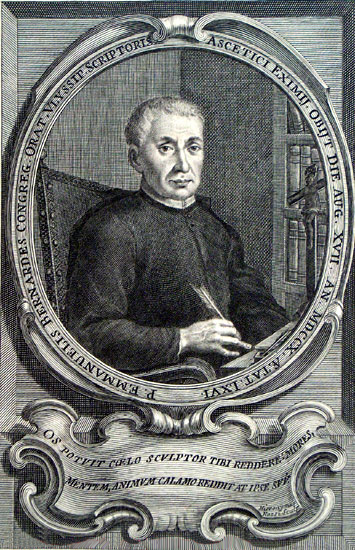
\includegraphics[width=0.5\textwidth]{media/bernardes}
\end{nscenter}

\begin{nscenter} \emph{Década 1} \end{nscenter}

Senhor Deus: eu sou a miséria, a ingratidão, a indignidade; sou um pecador vilíssimo, a quem não devia cobrir o Céu nem sustentar a Terra. Havei de mim misericórdia, e salvai-me por amor de vossa bondade.

Pai: pequei contra o Céu, e em vossa presença; não sou digno de me chamar filho vosso; fazei-me como qualquer de vossos mercenários.

Lavai-me, meu Senhor Jesus Cristo, nas correntes de vosso precioso Sangue; e limpai minha alma das manchas de todo o pecado.

Desgarrei-me como ovelha perdida. Que fora de mim, ó bom Pastor, se me não buscásseis, e tomásseis sobre vossos ombros?

Eis aqui está à vossa porta o pobre: eis aqui o leproso e cego, e tolhido, e coberto de inumeráveis chagas. Não necessitam de médico os sãos, mas os enfermos; vinde, e curai-me com vossa palavra, para glória de vosso nome.

Que era eu, Senhor, no meio de meus vícios, e fora de vossa graça, senão um cão morto, coberto das moscas dos demônios, que em minha podridão se cevavam. Vistes minha miséria, e vos apiedastes. Destes-me vida e misericórdia. Oh, bendito seja tal amor!

Inclinai, Senhor, para mim vossos amorosos olhos, e apagai meus pecados. Concedei-me a graça da renovação de meu espírito, com uma vida totalmente conforme à vossa lei.

Deus meu: proponho firmemente, com o auxílio de vossa graça, não admitir jamais ofensa vossa. Oh! não mais pecar, não mais desprezar vossos preceitos; guardá-los, sim, mais que as meninas dos meus olhos.

Senhor: alcance eu de vós esta mercê; que, no ponto em que certamente hei de cair de vossa graça, antes caia morto de repente; porque viver com injúria vossa pior morte é que a mesma morte, e maior desgraça que o inferno.

Jesus amorosíssimo, Jesus minha Redenção e remédio: de tantas lágrimas que andando neste mundo chorastes, dai-me uma para que amoleça este coração, e o derreta pelos olhos. Dai-me uma lágrima vossa, para que a apresente a vosso Eterno Padre em remissão de meus pecados.

\begin{nscenter} \emph{Década 2} \end{nscenter}

Não entreis, Senhor, em juízo com vosso servo; porque nenhum vivente se justificará diante de vós. De mil cargos que me fizerdes, não poderei responder a um só. Todo me entrego nos braços de vossa misericórdia.

Que maldade há no mundo tão execrável, que eu não esteja pronto para a cometer? Senhor, amarrai com as cadeias de vosso santo temor as fúrias de minha liberdade; porque sou capaz de tornar a crucificar-vos.

Isto me pasma, Senhor: como não respeitei vossa presença! Como não temi vossa indignação! Como me não compadeci de vossas dores! Como pisei vosso Sangue! Como não correspondi a tanto amor! Não pode haver maior cegueira.

Pecaste, alma minha: diz-me, agora, que fruto tiraste do teu pecado? Amaste as criaturas mais que ao Criador: que te ficou rendendo esta desordem? Perda da amizade de Deus, e do direito à sua glória, remorso de consciência, costume de tornar a pecar, escravidão ao demônio, reato da culpa, dívida da pena eterna. Oh, quem dera rios de lágrimas a meus olhos, para lamentar tão grave desgraça!

Vinde, vinde, Senhor, ao meu coração; formai um azorrague das cordas de vosso amor e temor, e lançai daqui todos os maus afetos que profanam a vossa casa.

Rogo-vos, meu Jesus, por aquele primeiro leite que bebeste nos peitos virginais de vossa Mãe Santíssima; e por aquelas sagradas primícias de vosso Sangue, que derramastes na Circuncisão, que não permitais que jamais caia de vossa graça nem esteja um ponto fora dela.

Pequei mais que o número das areias do mar. Porém, Senhor, as vossas misericórdias não têm número. Em vós ponho toda minha esperança: não padecerei confusão eterna.

Eu a pecar; vós, Senhor, a perdoar-me. Eu a fazer-vos injúrias; vós a fazer-me benefícios. O certo é, Senhor, que cada um obra como quem é. Bendita seja vossa paciência, que tanto me esperou.

Muito agravado estais de mim, e vos sobra razão. Oh, quem para aplacar-vos tivera as lágrimas de uma Madalena, as penitências de uma Egipcíaca, os gemidos de um Agostinho, a compunção de um S. Pedro!

Ah, pecador atrevido e infame! Tu foste o que açoutaste a JESUS, tu o que o coroaste de espinhos; o que lhe lançaste salivas no rosto, o que o pregaste na Cruz. Como te não confundes?

\begin{nscenter} \emph{Década 3} \end{nscenter}

Lembrai-vos, Senhor, que sou obra de vossas mãos; lembrai-vos que vos custei muito na Cruz. Não entregueis às bestas infernais as almas que vos confessam.

Não me dirás, alma minha, que males te fez teu Deus, para que assim o ofendesses? Acaso foi crime o morrer por ti de amor em uma Cruz? Porventura te agravou em querer salvar-te, e dar-te o Reino de sua Glória? Que razão posso dar, Senhor, do pecado, que é a mesma sem-razão? Misericórdia.

Ora pazes, Senhor; pazes para sempre; fiz mal, assim o confesso diante do Céu e da Terra. Não farei mais; perdoai-me por quem sois.

Vaidade de vaidades, e tudo vaidade. Que me pode render o amor do mundo, e todas suas cousas, senão deleite falso, que em um momento passa; tormento verdadeiro, que em uma eternidade não passa?

Que fará um desgraçado a quem a morte colheu em pecado mortal e sepultou nas profundezas? Oh, que gemidos! Oh, que ânsias! Oh, que remorsos! Oh, que desesperações! Oh, que incêndios! Tu não puderas já ser este? Quanto devo, Senhor, à vossa paciência! Bendita seja eternamente.

Não dissestes vós, Senhor, que havia grande festa e alegria no Céu quando algum pecador se convertia? Eia, amorosíssimo Jesus, fazei com vossa graça que seja eu o assunto desta alegria e festa.

Eis-me, aqui Senhor, que sou o filho pródigo, e dissipei a substância de vossa graça, e andei na região remota de vossa presença, apascentando os animais imundos de meus apetites; já torno para vossa graça, lançai-me os braços de vossa caridade.

Oh, banhe-me esse precioso Sangue, que com tanto amor derramastes pelos pecadores! Banhe-me todo com um perfeito batismo, e ficarei mais alvo que a neve.

Senhor Deus: aqui nesta vida me castigai, aqui me abrasai, contanto que me perdoeis eternamente. Não queirais, Senhor, entesourar contra mim vossa ira; não me guardeis para a outra vida a satisfação de vossa justiça.

Oh, horas preciosas dadas para servir e amar a Deus, e empregadas em ofendê-lo! Quem nunca houvera nascido para tanto mal! Ou quem de novo tornara a nascer, para o emendar!

\begin{nscenter} \emph{Década 4} \end{nscenter}

Oh, que cego andava eu Senhor, pois estava sem vós, e vós sois Luz! Oh, como ia errado, pois estava fora de vós, e vós sois Caminho! Oh, que nesciamente procedia, pois estava sem vós, e vós sois Sabedoria! Oh, como estava morto, pois estava sem vós, e vós sois vida!

Nada sou, nada valho, nada posso senão ofender-vos, e precipitar-me no inferno. Esta mesma verdade que agora conheço, se afastares vossa luz, me ficará oculta; e sobre tantas misérias minhas se acrescentará outra, de as não conhecer.

Oh, alma minha, em que te ocupas, em que te enredas? O teu Jesus coroado de espinhos, e tu de flores? Ele suando Sangue, e tu buscando refrigérios? Ele farto de opróbrios, tu faminta de honras? Oh, confusão! Mudemos de vida; tomemos a Cruz; sigamos os passos de Cristo.

De quantos bens me destes, Senhor, usei mal, e em ofensa vossa. Se me fizésseis Anjo, creio que já também fora demônio. Oh, quem tivera digno sentimento de tão enormes excessos, verdadeira dor de pecados tão graves!

O ofício que tomei, Senhor, foi o de pecar; e neste me exercitei com toda a diligência, estudando muito de propósito na maldade. Oh, que bem concordava isto com o fim para que vós me criastes, que é amar-vos, e gozar-vos eternamente! Só vós, que sois infinito em bondade, podereis sofrer tanto.

Onde me esconderei, Senhor, até que passe a vossa ira? Fugirei de vós para vós mesmo; de vós, reto Juiz, para vós, Pai clementíssimo. Em vossas chagas me recolho, que este é o sagrado que vale aos que vão fugindo à vossa justiça.

Oh, quanta foi até agora minha negligência e descuido! O tempo que me concedestes para a penitência, desperdicei-o; os auxílios de vossa graça, rejeitei-os; às vozes com que me chamáveis me fiz surdo. E agora, Senhor, que hei de fazer? Pesa-me de haver pecado; havei de mim misericórdia, misericórdia.

Que dormisse eu tão seguro sobre a vossa ofensa, pendurado do fio da vida sobre a boca do inferno! Grande temeridade a minha! Senhor, dai-me entendimento, e viverei amando-vos e servindo-vos.

Oh, se eu já desprezasse o mundo como ele merece! Oh, se metera debaixo dos pés todas as cousas terrenas! Oh, se somente fizera estimação das eternas!

Afastai, Senhor, vosso rosto de meus pecados; e apagai e extingui todas minhas iniqüidades. Criai em mim um coração novo; e renovai o espírito reto em minhas entranhas.

\begin{nscenter} \emph{Década 5} \end{nscenter}

Sei que hei de aparecer em vosso tribunal; sei que hei de dar-vos estreita conta de toda minha vida. Não me atrevo, Senhor, a suportar vossos olhos irados. Ordenai agora minha vida, de modo que não desmereça então vê-los benignos.

Aqui vos mostro, Senhor, todas minhas chagas. Vede como são muitas, como são profundas, como são envelhecidas? Ó médico Divino, sarai as minhas chagas com vossas; que, para os filhos de Adão estarem sãos, quis o Filho de Deus estar chagado.

Não te desalentes, Alma minha, com a enormidade e multidão de teus pecados. Espera sempre em Deus até à noite cerrada da tua morte; que em Deus há infinita misericórdia e redenção copiosa.

Ajudai-me, Deus Salvador meu; livrai-me por amor da glória do vosso nome. Não vos lembreis de minhas maldades; submergi-as no mar de vossa bondade imensa.

Olha, Alma minha, olha para teu Deus posto por ti em uma Cruz, eis ali o que perdoa, e apaga os teus pecados. Vê quanto padeceu por te salvar; vê com que fina caridade te ama. Guarda-te de jamais tornar a ofendê-lo.

A vós, Senhor, que sois dulcíssimo Esposo de minha alma, desprezei-vos; ao demônio, que é adúltero, fiz-lhe a vontade. Tomara morrer de sentimento de tão feia desordem. Tomara chorar de dia e de noite tão execranda maldade.

Que tenho eu com o mundo, que passa como figura? Que tenho eu com a carne, que murcha como flor? Que tenho com as cousas transitórias, que tudo é engano, perigo, trabalho, vaidade? Eia, eia, salvemos a alma nas tabuas da Cruz, fazendo penitência.

Oh, momento do qual pende a eternidade! Só quem te não considera te não teme. Abri-me, Senhor, os olhos da alma, não me suceda adormecer no letargo da morte eterna.

Senhor, aqui venho fugindo de meus inimigos: abri-me as portas de vossa misericórdia. Recolhei o vosso fugitivo, meu Deus; recolhei-me depressa, que meus inimigos me vêm ao alcance.

Dulcíssimo Jesus: o vosso soberano nome quer dizer Salvador; obrai em mim conforme vosso nome e salvai-me.
